\documentclass[a4paper]{article}
\usepackage[intlimits]{amsmath}
\usepackage[utf8]{inputenc}
\usepackage[margin=0.8in]{geometry}
\usepackage[numbered]{mcode}
\usepackage{graphicx}

\begin{document}

\centerline{\sc \large 3B.18: Teslatrasslet}
\vspace{.5pc}
\centerline{\sc Snurrig bana i magnetfält}
\vspace{2pc}

Uppgiften kan delas upp i tre delar. Del 1 går ut på att visa att
fältkomponenterna av en vektor 
$$
B(r, 0, z) = \frac{\mu_r\mu_0}{4\pi} \int_{-\pi}^\pi
\frac{\bf{i}(\varphi)\times\bf{s}(\varphi)}{s^3}ad\varphi
$$
med $\mu_0 = 4\pi \cdot 10^{-7}$,\ $\mathbf{i}(\varphi) = I_0(-sin\varphi,
cos\varphi, 0)$,\ $\mathbf{s}(\varphi) = \mathbf{p} - \mathbf{q} = (r -
acos\varphi, -asin\varphi, z)$ och $s = \|p - q\|_2 = \sqrt{(r - acos\varphi)^2
+ a^2sin^2\varphi + z^2}$ blir
$$
B_x = C\int_{-\pi}^\pi \frac{zcos\varphi}{s^3}d\varphi, \
B_y = 0,\
B_z = C\int_{-\pi}^\pi \frac{a - rcos\varphi}{s^3}d\varphi 
$$
där $C = \mu_rI_0a \cdot 10^{-7}$.

\vspace{1pc}
Det går att lösa enkelt utan nummeriska metoder. 
\begin{eqnarray*}
  B(r, 0, z) & = \frac{\mu_r\mu_0}{4\pi} \int_{-\pi}^\pi
  \frac{\bf{i}(\varphi)\times\bf{s}(\varphi)}{s^3}ad\varphi \\
  & = \frac{a\mu_r\mu_0}{4\pi} \int_{-\pi}^\pi
  \frac{\bf{i}(\varphi)\times\bf{s}(\varphi)}{s^3}d\varphi \\
  & = \frac{4\pi\mu_ra \cdot 10^{-7}}{4\pi} \int_{-\pi}^\pi 
  \frac{\bf{i}(\varphi)\times\bf{s}(\varphi)}{s^3}d\varphi \\
  & = \mu_ra \cdot 10^{-7} \int_{-\pi}^\pi
  \frac{\bf{i}(\varphi)\times\bf{s}(\varphi)}{s^3}d\varphi \\
  & = \mu_ra \cdot 10^{-7} \int_{-\pi}^\pi
  \frac{I_0(-sin\varphi, cos\varphi, 0)\times(r - acos\varphi, -asin\varphi,
  z)}{s^3}d\varphi \\
  & = \mu_rI_0a \cdot 10^{-7} \int_{-\pi}^\pi
  \frac{(-sin\varphi, cos\varphi, 0)\times(r - acos\varphi, -asin\varphi,
  z)}{s^3}d\varphi \\
  & = C \int_{-\pi}^\pi
  \frac{(-sin\varphi, cos\varphi, 0)\times(r - acos\varphi, -asin\varphi,
  z)}{s^3}d\varphi \\
  & = C \int_{-\pi}^\pi
  \frac{(zcos\varphi - 0, 0 - (-zsin\varphi), asin^2\varphi - cos\varphi(r -
  acos\varphi))}{s^3}d\varphi \\
  & = C \int_{-\pi}^\pi
  \frac{(zcos\varphi, zsin\varphi, asin^2\varphi + acos^2\varphi - rcos\varphi)}{s^3}d\varphi \\
  & = C \int_{-\pi}^\pi
  \frac{(zcos\varphi, zsin\varphi, a(sin^2\varphi + cos^2\varphi) - rcos\varphi)}{s^3}d\varphi \\
  & = C \int_{-\pi}^\pi
  \frac{(zcos\varphi, zsin\varphi, a - rcos\varphi)}{s^3}d\varphi \\
\end{eqnarray*}

Nu ser vi att $B_x = C\int_{-\pi}^\pi \frac{zcos\varphi}{s^3}d\varphi$ och $B_z
= C\int_{-\pi}^\pi \frac{a - rcos\varphi}{s^3}d\varphi $, men $B_y$ kräver lite mer analys.

\vspace{1pc}

Enligt beräkningen ovan gäller $B_y = C\int_{-\pi}^\pi
\frac{zsin\varphi}{s^3}d\varphi$. Dessutom vet vi att $y = 0$ eftersom vi
arbetar i punkten $p = (r, 0, z)$. Därför måste $sin\varphi = 0$, vilket medför
\begin{eqnarray*}
  B_y & = C\int_{-\pi}^\pi \frac{zsin\varphi}{s^3}d\varphi \\
      & = C\int_{-\pi}^\pi \frac{z \cdot 0}{s^3}d\varphi \\
      & = C \cdot 0 \\
      & = 0.
\end{eqnarray*}

Nu är del 1 nästan klar. Som uppgiftsförfattaren noterar har magnetfältet endast
komponenter i radiell- och z-led. Därför byter vi namn på $B_x$ till $B_r$, då
$y = 0$.

\clearpage
\centerline{\sc Fältlinjeberäkning}
\vspace{2pc}

Del 2 handlar om att nummeriskt lösa diffrentialekvationssystemet 

$$
dr/dv = B_r(r,z),\ dz/dv = B_z(r, z),\ r(0) = r_0,\ z(0) = 0.
$$
Det första problemet vi stöter på är att integralerna i $B_r$ och $B_z$ alltid
är lika med 0, eftersom funktionen vi söker bildar en oval med mittpunkt i
origo. Därför får vi ändra integreringsintervallet.

$$
C\int_{-\pi}^\pi \frac{zcos\varphi}{s^3}d\varphi = 4C\int_0^{\pi/2}
\frac{zcos\varphi}{s^3}d\varphi, \
C\int_{-\pi}^\pi \frac{a - rcos\varphi}{s^3}d\varphi = 4C\int_0^{\pi/2} \frac{a - rcos\varphi}{s^3}d\varphi 
$$

Nu kan ekvationssystemet lösas med Matlabs ODE.

\lstinputlisting{tesla.m}
\lstinputlisting{fp.m}

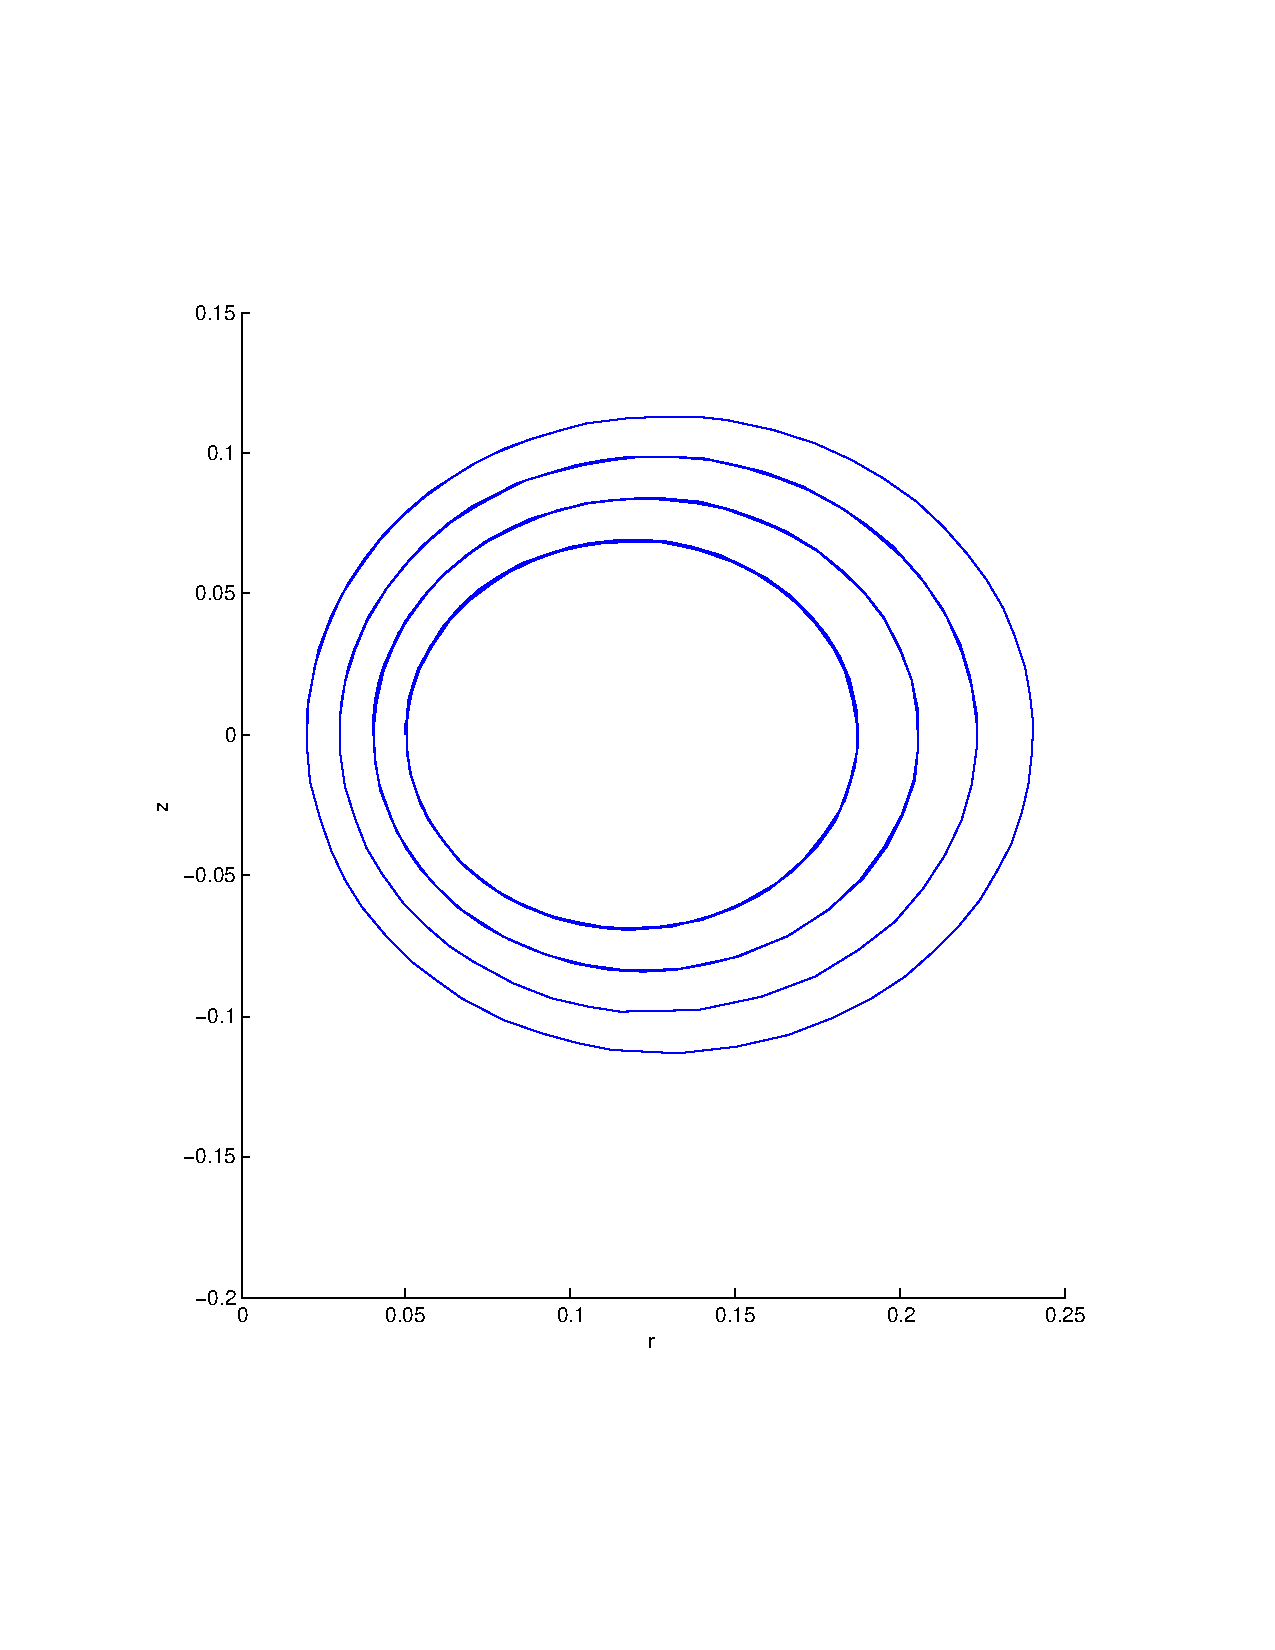
\includegraphics[scale=0.5]{ovals.pdf}

\clearpage
\centerline{\sc Beräkning av partikelbanor}
\vspace{2pc}

Del 3 handlar om ett nytt diffrentialekvationssystem. Vi söker en tidsberoende
partikelbana $\mathbf{s}(t) = (x(t), y(t), z(t))$ som beskrivs av
diffrentialekvationen $m\mathbf{\ddot{s}} = Q(\mathbf{\dot{s}} \times
\mathbf{B})$. I punkten $(x, y, z)$ har magnetfältet komponenterna
$$
B_x = \frac{x}{r}B_r,\ B_y = \frac{y}{r}B_r,\ B_z
$$
där $r = \sqrt{x^2 + y^2}$. Om vi inför $c_p = \frac{Q}{m}$ kan vi göra följande
härledning.
\begin{eqnarray*}
  m\mathbf{\ddot{s}} & = Q(\mathbf{\dot{s}} \times \mathbf{B}) \Leftrightarrow
  \\
  \mathbf{\ddot{s}} & = \frac{Q}{m}(\mathbf{\dot{s}} \times \mathbf{B}) = 
  \\
  \mathbf{\ddot{s}} & = c_p(\mathbf{\dot{s}} \times \mathbf{B}) = 
  \\
  (\ddot{x}, \ddot{y}, \ddot{z})& = c_p((\dot{x},\dot{y},\dot{z}) \times
  (\frac{x}{r}B_r,\frac{y}{r}B_r,B_z)) = 
  \\
  (\ddot{x}, \ddot{y}, \ddot{z})& = c_p(\dot{y}B_z - \dot{z}B_y, 
  \dot{z}B_x - \dot{x}B_z, \dot{x}B_y - \dot{y}B_x) = 
  \\
  (\ddot{x}, \ddot{y}, \ddot{z})& = (c_p(\dot{y}B_z - \dot{z}B_y), 
  c_p(\dot{z}B_x - \dot{x}B_z), c_p(\dot{x}B_y - \dot{y}B_x))
\end{eqnarray*}
Alltså blir komponenterna 
$$
\ddot{x} = c_p(\dot{y}B_z - \dot{z}B_y),\ \ddot{y} = c_p(\dot{z}B_x -
\dot{x}B_z),\ \ddot{z} = c_p(\dot{x}B_y - \dot{y}B_x).
$$
För att kunna lösa systemet med ode45 behöver vi skriva om systemet till en
första ordningens diffrentialekvationssystem. Därför inför vi betäckningarna

\begin{align*}
  u_1 &= x,\ u_2 = \dot{x}, & \dot{u_1} = u_2,\ \dot{u_2} = c_p(v_2B_z -
  w_2B_y),\\
  v_1 &= y,\ v_2 = \dot{y},& \dot{v_1} = v_2,\ \dot{v_2} = c_p(w_2B_x - u_2B_z),\\
  w_1 &= z,\ w_2 = \dot{z},& \dot{w_1} = w_2,\ \dot{w_2} = c_p(u_2B_y - v_2B_x).\\
\end{align*}
Nu kan vi lösa systemet med hjälp av startvärdena nedan.
\begin{align*}
  x(0) &= 1.2a, & \dot{x}(0) = 0,\\
  y(0) &= 0, & \dot{y}(0) = v_0,\\
  z(0) &= 0.15a, & \dot{z}(0) = 0
\end{align*}
där $v_0 = 200000$ och $c_p = 2 \cdot 10^7$.
\end{document}
